%==================================================
%      PREAMBOLO e DICHIARAZIONI INIZIALI
%==================================================
\documentclass[10pt,oneside,a4paper]{article}

\usepackage[latin1]{inputenc} 
\usepackage[italian]{babel}
\usepackage[T1]{fontenc}
\usepackage{siunitx} %Inserisce automaticamente i dati con le unit�  di misura correttamente formattate del SI (utilizzo: \SI{0.82}{m^2}, in generale \SI{misura con il punto decimale}{unit�  di misura})
\sisetup{output-decimal-marker = {.}, separate-uncertainty = true, input-uncertainty-signs = \pm, detect-weight=true, detect-family=true} %per usare SI con il punto decimale
\usepackage{listings} %Per citare codice informatico formattandolo correttamente
\usepackage{amsmath,amsthm,verbatim,amssymb,amsfonts,amscd,graphicx,mathtools}
\usepackage[makeroom]{cancel}
\newcommand{\abs}[1]{\left\lvert\,#1\,\right\rvert}
\usepackage{geometry}
\usepackage{epigraph}
\usepackage{booktabs}	%tabelle migliorate
\usepackage{tablefootnote}	%note a pi� di pagina in tabella
\usepackage{threeparttable} %tabella con note a pi� di tabella
\usepackage{caption}	%descrizione per figure
\usepackage{dblfnote}
\captionsetup{tableposition=top,figureposition=bottom,font=small} %setup descrizione
\usepackage{float}
\usepackage{esvect} %vettori
\usepackage{longtable} %tabelle lunghe
\usepackage[dvipsnames]{xcolor}
\definecolor{sepia}{HTML}{80002A}
\usepackage[colorlinks=true, citecolor=black, linkcolor=sepia, urlcolor=black]{hyperref}
\usepackage{mathrsfs}
\usepackage{circuitikz}
\tikzset{
  font={\fontsize{7pt}{12}\selectfont}}
\ctikzset{bipoles/resistor/height=0.2}
\ctikzset{bipoles/resistor/width=0.4}
\ctikzset{bipoles/diode/height=0.3}
\ctikzset{bipoles/diode/width=0.3}
\ctikzset{tripoles/american nand port/height=0.7}
\ctikzset{tripoles/american nand port/width=0.8}
\usepackage{enumitem} %Liste senza spazi verticali
\setlist{noitemsep}
\usepackage{amsmath}


\interfootnotelinepenalty=10000


\usepackage{multicol}
\newenvironment{Figure}
  {\par\medskip\noindent\minipage{\linewidth}}
  {\endminipage\par\medskip}

\newcommand{\var}{\operatorname{var}}
\newcommand{\cov}{\operatorname{cov}}


\usepackage{listings} %Per inserire codice
\lstnewenvironment{codice_c}[1][]
{\lstset{basicstyle=\small\ttfamily, columns=fullflexible,
keywordstyle=\color{red}\bfseries, commentstyle=\color{blue},
language=C, basicstyle=\small,
numbers=left, numberstyle=\tiny,
stepnumber=2, numbersep=5pt, frame=shadowbox,  showstringspaces=false, #1}}{}

%==================================================
%                  PRIMA PAGINA
%==================================================

\title{\textsc{\textbf{Esercitazione 7}: Costruzione di un ADC}}
\author{\small{G. Galbato Muscio} \and \small{L. Gravina} \and \small{L. Graziotto}}
\date{4 Dicembre 2018}

\begin{document}
	\begin{figure}
		\centering
		
\includegraphics[scale=0.5, trim={2.8cm 8.9cm 0 9cm}, clip]{logo.png}
	\end{figure}
	\maketitle
	\begin{center} 
		\fbox{{\fontsize{12pt}{8mm}\textsc{Gruppo 11}}} \\
	\end{center}
\hrule
\vspace{0.5cm}
\renewcommand{\abstractname}{Abstract}
\begin{abstract}
Si realizza un \emph{analog to digital converter}, utilizzando un contatore a 4 bit realizzato con l'integrato 7493 e costruendo un DAC a pesiera a 4 ingressi e un comparatore, con l'amplificatore operazionale LM358, e un adattatore di livello logico, con l'integrato 74LS00.
\end{abstract}
\vspace{4cm}
\tableofcontents %Indice
\newpage


\pagebreak


\begin{multicols}{2}
%==================================================
%             INTRODUZIONE
%==================================================
\section{Introduzione}
\begin{figure*}[t]
\caption{Circuito completo dell'ADC}
\label{fig:complete_circuit}
\centering
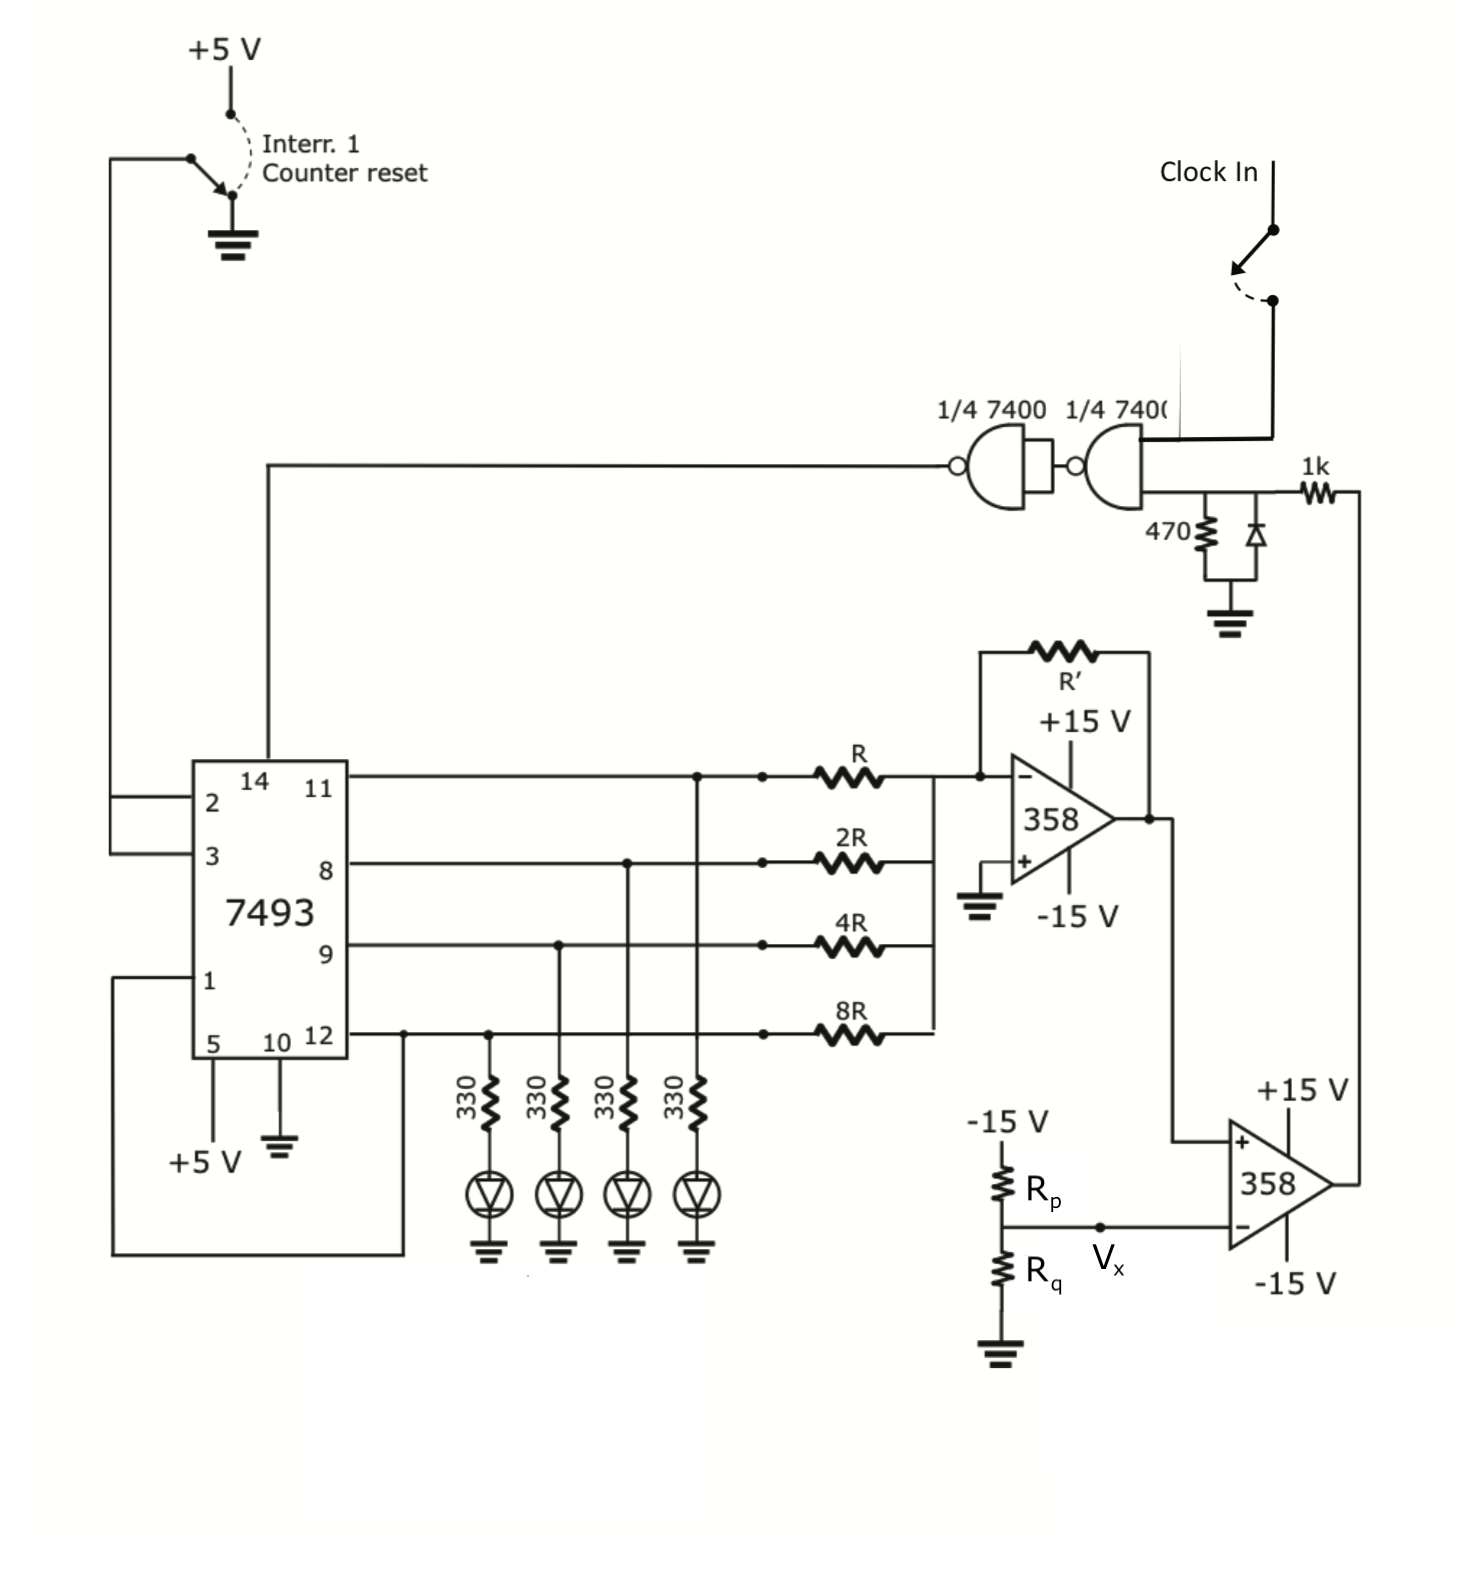
\includegraphics[width=0.7\linewidth]{completo}
\end{figure*}



Si realizza un convertitore analogico-digitale (ADC) a 4 bit, ossia un dispositivo che converte una tensione di ingresso $V_x$ in un numero binario a 4 bit ad essa proporzionale. Si riporta in Figura~\ref{fig:complete_circuit} il circuito completo, nel quale � possibile distinguere un contatore a 4 bit (realizzato con l'integrato 7493), un comparatore d'ingresso realizzato con un op-amp, attraverso il quale verr� fornita al circuito la tensione $V_x$, un convertitore digitale-analogico (DAC) a pesiera a 4 ingressi e un adattatore di livello logico.

La tensione da convertire, $V_x$, sar� negativa e tale che
\[
\SI{- 5}{V} \leq V_x \leq 0
\]
ed � ottenuta mediante un partitore costruito con un trimmer, collegato alla tensione di \SI{-15}{V} erogata dal generatore. 

%==================================================
%             CONTATORE A 4 BIT
%==================================================
\section{Contatore a 4 bit}\label{sec:counter}
Si realizza un contatore a 4 bit utilizzando l'integrato 7493; si riporta in Figura~\ref{fig:counter} il circuito corrispondente. Il componente � alimentato con una tensione continua di \SI{5}{V} erogata da uno dei due generatori, e si collegano entrambi gli ingressi di \texttt{RESET}, mediante un interruttore, alternativamente a massa o a \SI{5}{V}, per azzerare manualmente il contatore. 

\begin{Figure}
\captionof{figure}{Contatore a 4 bit}
\label{fig:counter}
\centering
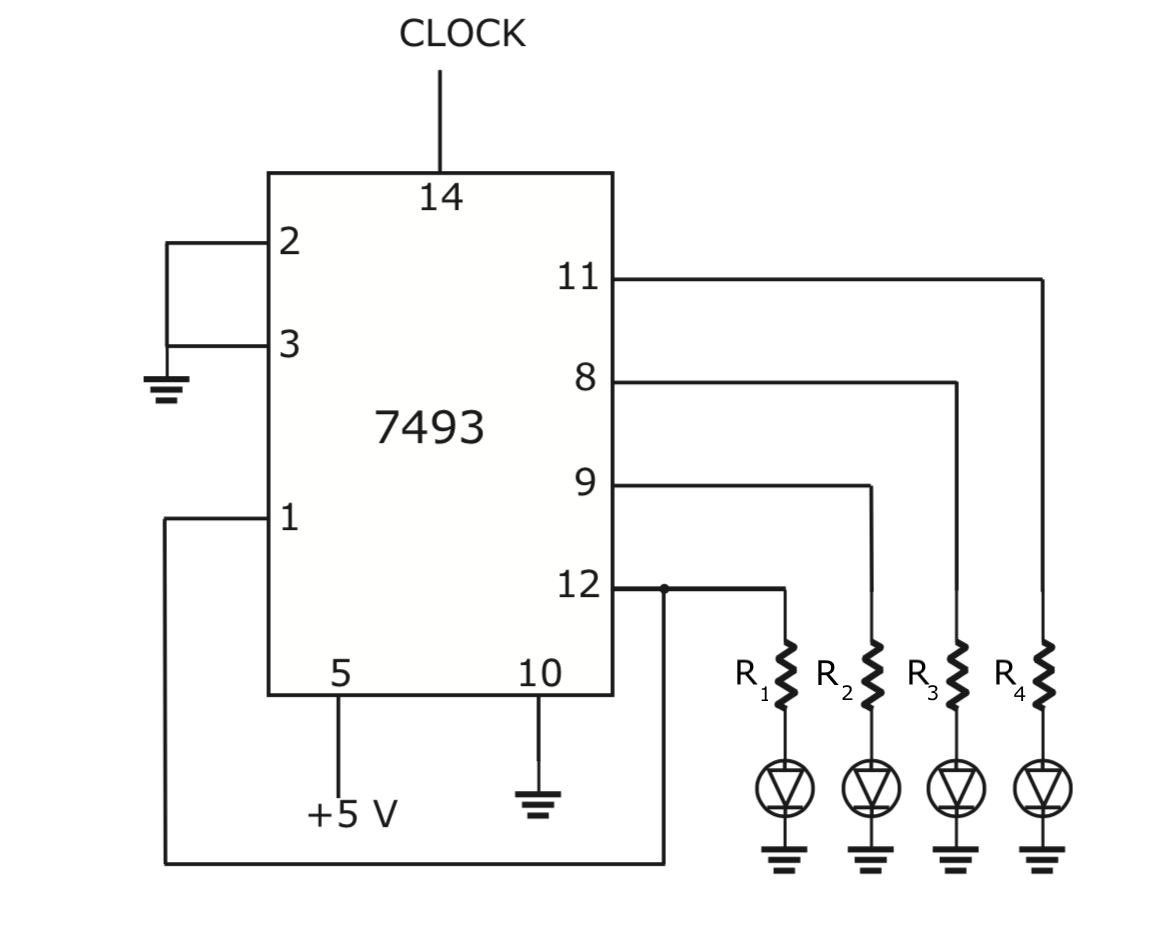
\includegraphics[width=\linewidth]{contatore}
\end{Figure}

Si connette inoltre il pin \texttt{1} al pin \texttt{12} in modo da fornire al secondo flip-flop interno all'integrato il segnale in uscita dal primo flip-flop come ingresso di clock.

Alle uscite vengono collegati, protetti da resistenze dell'ordine dei \SI{500}{\ohm}, dei led, al fine di verificare il corretto funzionamento del dispositivo. Essi sono infatti ordinati dall'output relativo al bit pi� significativo a quello relativo al bit meno significativo, e la loro progressiva e ordinata accensione sar� indice di funzionamento. Si invia dunque all'ingresso di \texttt{CLOCK} un'onda quadra TTL con frequenza di \SI{111 \pm 111}{Hz} e ampiezza variabile tra \SI{0}{} e \SI{111}{V}\footnote{Come nella precedente esperienza, si osserva che il generatore di segnali non genera un'onda TTL tra $0$ e \SI{5}{V}, bens� oscillante tra i valori indicati.}, mediante il generatore di segnali.

Si osserva che, come previsto, i LED si accendono in successione per formare la sequenza di numeri da $0$ a $15$. Le resistenze usate a protezione dei LED, misurate con il multimetro, sono:
\begin{itemize} %Lo spazio verticale � stato tolto con \setlist{noitemsep} nell'header, rimuovere quella riga per avere una lista classica
	\item[--] $R_1 = \SI{111 \pm 111}{\ohm}$;
	\item[--] $R_2 = \SI{111 \pm 111}{\ohm}$;
	\item[--] $R_3 = \SI{111 \pm 111}{\ohm}$;
	\item[--] $R_4 = \SI{111 \pm 111}{\ohm}$.
\end{itemize}

Si misurano inoltre i livelli di tensione in uscita al contatore mediante il multimetro: si resetta il contatore a 0000 e quindi, mediante un clock manuale, lo si porta a 1111. Si riportano in Tabella~\ref{tab:counter} le misure di tensione per i livelli logici alto e basso per i quattro output.

\begin{center}
\captionof{table}{Misure di tensione sul contatore}
\label{tab:counter}
\begin{tabular}{c|c|c}
Output & $V$ a 0 logico [\SI{}{V}] & $V$ a 1 logico [\SI{}{V}] \\
\hline
      $Q_0$ &        111 &         111  \\
      $Q_1$ &        111 &         111  \\
      $Q_2$ &        111 &         111  \\
      $Q_3$ &        111 &         111  \\
\hline
\end{tabular}
\end{center}

%==================================================
%             DAC A 4 BIT
%==================================================
\section{DAC a 4 bit}
Si costruisce un convertitore digitale-analogico (DAC) invertente a pesiera, utilizzando l'amplificatore operazionale LM358, alimentato con tensione di $\pm \SI{15}{V}$, erogata dal generatore. Si scelgono le resistenze in modo da avere un'uscita compresa nella massima dinamica possibile per l'operazionale, ricordando che in ingresso si fornir� un livello logico TTL, che, da quanto visto nella sezione precedente, avr� come valore di tensione corrispondente a 0 logico \SI{111}{V}, e tensione corrispondente a 1 logico al massimo \SI{111}{V}. Inoltre i valori delle resistenze saranno scelti dell'ordine del \SI{}{\kilo\ohm}, in modo da evitare eccessi di corrente. 

Si riporta in Figura~\ref{fig:dac} il circuito realizzato.

\begin{Figure}
\captionof{figure}{Convertitore digitale-analogico}
\label{fig:dac}
\centering
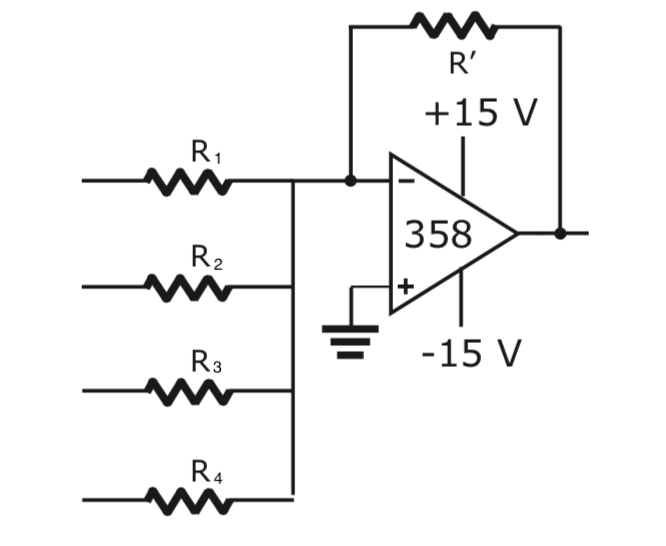
\includegraphics[width=\linewidth]{dac}
\end{Figure}

Per compiere la regolazione della rete pi� precisa possibile, si sceglie di utilizzare un resistore fisso in corrispondenza di $R_1$, e di utilizzare dei trimmer in luogo di $R_2$, $R_3$ e $R_4$, tali da soddisfare le seguenti relazioni
\[
\begin{aligned}
R_2 &= 2 R_1; \\
R_3 &= 4 R_1; \\
R_4 &= 8 R_1.
\end{aligned}
\] 
Ricordando che in questo caso la risposta dell'op-amp �
\[
V_o = -\frac{R'}{8R}\big[V(Q_0) + 2V(Q_1) + 4V(Q_2) + 8V(Q_3)\big],
\]
e che si ha, per quanto visto prima, al massimo $V(Q_i) = \SI{111}{V} \equiv V_\text{in}^\text{max}$, si ottiene la relazione
\[
V_o = -\frac{R'}{8R} \cdot 15 \cdot V_\text{in}^\text{max},
\] 
che invertita pone una condizione sui valori di $R'$ ed $R$ (e conseguentemente sui valori impostati sui trimmer), poich� la tensione di uscita massima dev'essere minore di \SI{15}{V}, in modo da rimanere entro la dinamica dell'amplificatore invertente:
\[
\frac{R'}{R} < \frac{8}{V_\text{in}^\text{max}} = \frac{8}{111} = 111.
\]
Pertanto si scelgono per le resistenze i valori seguenti, misurati con il multimetro:

\begin{itemize} %Lo spazio verticale � stato tolto con \setlist{noitemsep} nell'header, rimuovere quella riga per avere una lista classica
	\item[--] $R_1 = \SI{111 \pm 111}{\ohm}$;
	\item[--] $R_2 = \SI{111 \pm 111}{\ohm}$;
	\item[--] $R_3 = \SI{111 \pm 111}{\ohm}$;
	\item[--] $R_4 = \SI{111 \pm 111}{\ohm}$;
	\item[--] $R' = \SI{111 \pm 111}{\ohm}$.
\end{itemize}

Si verifica quindi che il circuito si comporti correttamente come un sommatore invertente, osservando l'uscita al canale \texttt{CH2} dell'oscilloscopio e fornendo manualmente tensioni di \SI{111}{V} agli ingressi, con un partitore di tensione.

Si collegano quindi agli ingressi del DAC le uscite del contatore realizzato nella Sezione~\ref{sec:counter}; quindi si fornisce al contatore un clock mediante un'onda quadra TTL di frequenza \SI{111}{Hz}, e ampiezza variabile tra i valori gi� discussi precedentemente. Si riporta in Figura~\ref{fig:verifica_tensione_dac} un'istantanea dell'oscilloscopio per questa configurazione: al canale \texttt{CH1} vi � l'onda quadra di clock, mentre al \texttt{CH2} l'uscita del DAC. Si osserva come essa sia decrescente, in quanto l'amplificatore � invertente, e presenti un andamento della tensione \emph{a gradini}.

%\begin{Figure}
%	\begin{center}
%	\includegraphics[width=\linewidth]{}
%	\captionof{figure}{Istantanea dell'oscilloscopio per la tensione di uscita del DAC}
%	\label{fig:verifica_tensione_dac}
%	\end{center}
%\end{Figure}

Per misurare l'altezza di tali \emph{gradini}, si procede impostando manualmente il clock, e facendo avanzare il conteggio da 0 a 15; si misurano quindi con il multimetro i valori della tensione in output all'op-amp. Si riportano in Tabella~\ref{tab:verifica_dac} i punti sperimentali trovati, e la stima dell'altezza di ciascun gradino come differenza del valore misurato con quello precedente.

\begin{center}
\captionof{table}{Misure sul circuito DAC}
\label{tab:verifica_dac}
\begin{tabular}{c|c|c}
Contatore & $V_\text{out}$ [\SI{}{V}] & $\Delta V_\text{out}$ [\SI{}{mV}] \\
\hline
      0 &        111 &         111  \\
      1 & 		111 &         111  \\
\hline
\end{tabular}
\end{center}

Si riporta inoltre in Figura~\ref{fig:tensione_DAC} l'andamento della tensione in uscita dal DAC in funzione del numero dato dal contatore. Si osserva che essa ha pendenza negativa di \SI{111}{V}, come previsto dalla modalit� invertente, e che al numero $15$ corrisponde un'uscita di \SI{-15}{V}, a conferma della copertura con la massima sensibilit� dell'intero range a disposizione dell'amplificatore. Inoltre, la linearit� dell'andamento � confermata dalla stima del chi-quadro $111$, contro un numero di gradi di libert� di $14$.

%\begin{Figure}
%	\begin{center}
%	\includegraphics[width=\linewidth]{}
%	\captionof{figure}{Tensione in uscita al DAC in funzione del numero in ingresso}
%	\label{fig:tensione_DAC}
%	\end{center}
%\end{Figure}

%==================================================
%             COMPARATORE ANALOGICO
%==================================================
\section{Comparatore analogico}
Si realizza un comparatore analogico utilizzando un amplificatore operazionale LM358, alimentato con una tensione di $\pm \SI{15}{V}$; il circuito � il seguente.

\begin{center}
\begin{circuitikz}
\draw (0,0) node[op amp, yscale=-1] (opamp) {}
(opamp.+) -| ++(-1,1) node[above] {Uscita del DAC} 
(opamp.out) node[circ]{} node[right] {$V_\text{out}$}
(opamp.-) -- ++(-1,0) node[circ]{} node[above]{$V_x$} -- ++(-1,0) node[](trimmer){} to[R=$R_1$] ++(0,1.5) node[above]{\SI{-15}{V}}
(trimmer) to[R=$R_2$] ++(0,-1.5) node[ground]{}
;\end{circuitikz}
\end{center}

La tensione $V_x$ viene dunque prelevata da quella a \SI{-15}{V} fornita dal generatore mediante un trimmer, di resistenze $R_1$, $R_2$ variate mediante un cacciavite:
\[
V_x = \SI{-15}{V} \frac{R_2}{R_1 + R_2}.
\]

Il trimmer complessivamente prevede una resistenza $R_1 + R_2 = \SI{111}{\kilo\ohm}$.

Il funzionamento del comparatore prevede che fintanto che la tensione in uscita dal DAC � maggiore di $V_x$ il contatore continui ad incrementare il conteggio; non appena la tensione in uscita dal DAC diventa minore di $V_x$, il contatore blocca il conteggio, mediante un altro circuito di stop che sar� analizzato nel seguito. � evidente che la massima tensione comparabile, e dunque convertibile in digitale, $V_x$ � proprio pari alla massima tensione d'uscita del DAC.

%==================================================
%             ADATTAMENTO TTL E STOP DEL CLOCK
%==================================================
\section{Adattamento TTL e stop del clock}
Si realizza mediante le porte NAND dell'integrato 74LS00 e un diodo 1N4148 l'adattatore di tensione TTL che permette inoltre lo stop del clock quando l'uscita del comparatore analogico si porta a \SI{-15}{V}. Il circuito � il seguente.

\begin{circuitikz}
\draw (0,0) node[american nand port, xscale=-1] (nand) {}
(nand.in 1) to[short] (nand.in 2)  
(nand.in 1 |- nand.out) to [short,-] ++(0,0)
(nand.out) -- ++(-1,0) node[left]{Al contatore}
(nand.in 1 |- nand.out) to [short,-] (1.3,0) node[american nand port, xscale=-1] (nand2) {}
(nand2.in 1) -| ++(1,1) node[above]{Al \texttt{CLOCK}}
(nand2.in 2) -- ++(1.3,0) to[R=$R_1$] ++(1.2, 0) -| ++(0.1,-2) node[below]{Output comparatore}
(nand2.in 2) ++(0.4,0) node[](base){} ++(0,-1) node[](top){} -- ++(0.25,0) node[ground]{} -- ++(0.25,0) to[diode] ++(0,1)
(top) to[R=$R_2$] (base)
;\end{circuitikz}

I resistori hanno valori, misurati con il multimetro, di

\begin{itemize} %Lo spazio verticale � stato tolto con \setlist{noitemsep} nell'header, rimuovere quella riga per avere una lista classica
	\item[--] $R_1 = \SI{111 \pm 111}{\ohm}$;
	\item[--] $R_2 = \SI{111 \pm 111}{\ohm}$,
\end{itemize}
e costituiscono un partitore che riporta a \SI{5}{V} l'ingresso della porta NAND. Il diodo � inserito in modo da portarsi in conduzione quando l'uscita del comparatore commuta a \SI{-15}{V}: in tale caso, il potenziale del catodo diventa di \SI{-0.2}{V}, ossia 0 logico, perci� tramite le porte NAND, l'ingresso di clock del contatore si porter� anch'esso a 0 logico, bloccando il conteggio al numero corrispondente alla conversione digitale discreta della tensione analogica continua $V_x$. 

%==================================================
%             CIRCUITO COMPLETO
%==================================================
\section{Circuito completo}
Si completa il circuito unendo le diverse componenti realizzate nelle sezioni precedenti. 

Si connette quindi l'ingresso di \texttt{CLOCK} dell'adattatore TTL ad un segnale di onda quadra prelevato dall'uscita TTL del generatore di segnali, con frequenza \SI{111}{Hz}. Si azzera manualmente il contatore e si imposta un valore di tensione $V_x$ ($\SI{-5}{V}<V_x<\SI{0}{V}$) agendo sul trimmer del partitore; si pone l'interruttore di reset nuovamente a massa, in modo da permettere il funzionamento del contatore, e si legge il numero corrispondente al valore digitale della tensione mediante i LED.

Variando i valori delle resistenze del partitore, si pu� inviare in ingresso una tensione $V_x$ differente: si riportano dunque in Tabella~\ref{tab:calibrazioneADC} i valori di $V_x$ e le relative uscite digitali. Si riporta nel grafico di Figura~\ref{fig:calibrazioneADC} l'andamento dell'uscita digitale in funzione dell'ingresso di tensione analogica $V_x$. Si osserva la linearit� dei dati sperimentali, dai quali, mediante interpolazione, si ricava una pendenza di \SI{111}{V^{-1}} e un'intercetta \SI{111}{}. Il chi-quadro di $111$, prossimo al valore atteso di $14$, conferma la bont� del fit.

\begin{table*}
\captionof{table}{Misure per la calibrazione dell'ADC}
\label{tab:calibrazioneADC}
\begin{center}
\begin{tabular}{c|c|c|c}
$R_1$ [\SI{}{\kilo\ohm}] & $R_2$ [\SI{}{\kilo\ohm}] & $V_x$ [\SI{}{V}] & Contatore \\
\hline
\hline
\end{tabular}
\end{center}
\end{table*}

%\begin{Figure}
%	\begin{center}
%	\includegraphics[width=\linewidth]{}
%	\captionof{figure}{Uscita digitale in funzione del valore di tensione analogica $V_x$}
%	\label{fig:calibrazioneADC}
%	\end{center}
%\end{Figure}



\end{multicols}
\newpage
\section{Appendice}


%ESEMPIO DI FIGURA
%\begin{Figure}
%	\begin{center}
%	\includegraphics[width=\linewidth]{comune.png}
%	\captionof{figure}{Istantanea dell'oscilloscopio per l'amplificatore differenziale, misura di $A_c$}
%	\label{fig:Ac_differenziale}
%	\end{center}
%\end{Figure}


%ESEMPIO DI TABELLA
%\begin{center}
%\captionof{table}{Misure per la stima di $A_c$}
%\label{tab:Ac_differenziale}
%\begin{tabular}{c|c|c|c}
%$f$ [\SI{}{Hz}] & $V_i$ [\SI{}{V}] & $v_o$ [\SI{}{mV}] & $A_c = v_o / V_i$ \\
%\hline
%      149.5 &        3.90 &         11.3 & 2.90e-03 \\
%      222.0 &        3.90 &         11.5 & 2.95e-03 \\
%      281.0 &        3.90 &         11.8 & 3.03e-03 \\
%      359.0 &        3.90 &         11.8 & 3.03e-03 \\
%      461.0 &        3.90 &         12.2 & 3.13e-03 \\
%\hline
%\end{tabular}
%\end{center}



\end{document}